\chapter{Boolean Functions}\label{ch04}

\begin{tcolorbox}[colback=blue!5!white,colframe=blue!75!black]
	% Upper half of box: my "title" area
	\textcolor{blue}{\textbf{What To Expect}}
	% Lower half of the box: the content
	\tcblower
	In 1854, George Boole introduced an algebra system designed to work with binary (or base 2) numbers, but he could not have foreseen the immense impact his work would have on systems like telephony and computer science. This chapter includes the following topics.

	\begin{itemize}
		\item Developing and using the primary Logic Functions: AND, OR, NOT
		\item Developing and using the secondary Logic Functions: XOR, XNOR, NAND, NOR, Buffer
		\item Developing and using the univariate Boolean Algebra Properties: Identity, Idempotence, Annihilator, Complement, Involution
		\item Developing and using the multivariate Boolean Algebra Properties: Commutative, Associative, Distributive, Absorption, Adjacency
		\item Analyzing circuits using DeMorgan's Theorem
	\end{itemize}
\end{tcolorbox}


\section{Introduction to Boolean Functions}

Before starting a study of Boolean functions, it is important to keep in mind that this mathematical system concerns electronic components that are capable of only two states: \emph{True} and \emph{False} (sometimes called \emph{High-Low} or $ 1 $ - $ 0 $). Boolean functions are based on evaluating a series of \emph{\emph{True}-\emph{False}} statements to determine the output of a circuit.

For example, a Boolean expression could be created that would describe ``If the floor is dirty OR company is coming THEN I will mop.'' (The things that I do for visiting company!) These types of logic statements are often represented symbolically using the symbols $ 1 $ and $ 0 $, where $ 1 $ stands for \emph{True} and $ 0 $ stands for \emph{False}. So, let ``Floor is dirty'' equal $ 1 $ and ``Floor is not dirty'' equal $ 0 $. Also, let ``Company is coming'' equal $ 1 $ and ``Company is not coming'' equal $ 0 $. Then, ``Floor is dirty OR company is coming'' can be symbolically represented by $ 1 $ \textsf{OR} $ 1 $. Within the discipline of Boolean algebra, common mathematical symbols are used to represent Boolean expressions; for example, Boolean \textsf{OR} is frequently represented by a mathematics plus sign, as shown below. 

% Using + to represent OR
\begin{align}
  \label{04eq01}
  0 + 0 &= 0 \\
  \nonumber
  0 + 1 &= 1 \\
  \nonumber
  1 + 0 &= 1 \\
  \nonumber
  1 + 1 &= 1
\end{align}

These look like addition problems, but they are not (as evidenced by the last line). It is essential to keep in mind that these are merely symbolic representations of \emph{True}-\emph{False} statements. The first three lines make perfect sense and look like elementary addition. The last line, though, violates the principles of addition for real numbers; but it is a perfectly valid Boolean expression. Remember, in the world of Boolean algebra, there are only two possible values for any quantity: $ 1 $ or $ 0 $; and that last line is actually saying \emph{True \textsf{OR} True is True}. To use the dirty floor example from above, ``The floor is dirty'' (\emph{True}) OR ``Company is coming'' (\emph{True}) SO ``I will mop the floor'' (\emph{True}) is symbolized by: $ 1 + 1 = 1 $. This could be expressed as \emph{T \textsf{OR} T SO T}; but the convention is to use common mathematical symbols; thus: $ 1 + 1 = 1 $. 

Moreover, it does not matter how many or few terms are \textsf{OR} ed together; if just one is \emph{True}, then the output is \emph{True}, as illustrated below:

\begin{align}
  \label{04eq02}
  1 + 1 + 1 &= 1 \\
  \nonumber
  1 + 0 + 0 + 0 + 0 &= 1 \\
  \nonumber
  1 + 1 + 1 + 1 + 1 + 1 &= 1
\end{align}

Next, consider a very simple electronic sensor in an automobile: IF the headlights are on AND the driver's door is open THEN a buzzer will sound. In the same way that the plus sign is used to mathematically represent \textsf{OR} , a times sign is used to represent \textsf{AND} . Therefore, using common mathematical symbols, this automobile alarm circuit would be represented by $ 1 X 1 = 1 $. The following list shows all possible states of the headlights and door:

% Using X to represent AND
\begin{align}
  \label{04eq03}
  0 X 0 &= 0 \\
  \nonumber
  0 X 1 &= 0 \\
  \nonumber
  1 X 0 &= 0 \\
  \nonumber
  1 X 1 &= 1
\end{align}

The first row above shows ``\emph{False} (the lights are not on) AND \emph{False} (the door is not open) results in \emph{False} (the alarm does not sound)''. For \textsf{AND}  logic, the only time the output is \emph{True} is when all inputs are also \emph{True}; therefore: $ 1 X 1 X 1 X 1 X 0 = 0 $. In this way, Boolean \textsf{AND}  behaves somewhat like algebraic multiplication.

Within Boolean algebra's simple \emph{True}-\emph{False} system, there is no equivalent for subtraction or division, so those mathematical symbols are not used. Like real-number algebra, Boolean algebra uses alphabetical letters to denote variables; however, Boolean variables are always CAPITAL letters, never lower-case, and normally only a single letter. Thus, a Boolean equation would look something like this:

\begin{align}
  \label{04eq04}
  A + B &= Y 
\end{align}

As Boolean expressions are realized (that is, turned into a real, or physical, circuit), the various operators become \emph{gates}. For example, the above equation would be realized using an \textsf{OR}  gate with two inputs (labeled $ A $ and $ B $) and one output (labeled $ Y $). 

Boolean algebra includes three primary and four secondary logic operations (plus a Buffer, which has no logic value), six univariate, and six multivariate properties. All of these will be explored in this chapter.

\section{Primary Logic Operations}\label{0401}
\subsection{AND}

An \textsf{AND}  gate is a Boolean operation that will output a logical one, or \emph{True}, only if all of the inputs are \emph{True}. As an example, consider this statement: ``If I have ten bucks AND there is a good movie at the cinema, then I will go see the movie.'' In this statement, ``If I have ten bucks'' is one variable and ``there is a good movie at the cinema'' is another variable. If both of these inputs are \emph{True}, then the output variable (``I will go see the movie'') will also be \emph{True}. However, if either of the two inputs is \emph{False}, then the output will also be \emph{False} (or, ``I will not go see the movie''). Of course, if I want popcorn, I would need another ten spot, but that is not germane to this example. When written in an equation, the Boolean \textsf{AND}  term is represented a number of different ways. One method is to use the logic \textsf{AND} symbol as found in Equation \ref{BF:eq:and_symbol_logical}.

\begin{align}
  \label{04eq05}
  A \wedge B &= Y 
\end{align}

One other method is to use the same symbols that are used for multiplication in traditional algebra; that is, by writing the variables next to each other, with parenthesis, or, sometimes, with an asterisk between them, as in Equation \ref{04eq06}.

% Using X to represent AND
\begin{align}
  \label{04eq06}
  AB &= Y \\
  \nonumber
  (A)(B) &= Y \\
  \nonumber
  A * B &= Y
\end{align}

\marginpar{The multiplication symbols $ X $ and $\bullet$ (dot) are not commonly used in digital logic equations.} Logic \textsf{AND} is normally represented in equations by using an algebra multiplication symbol since it is easy to type; however, if there is any chance for ambiguity, then the Logic \textsf{AND}  symbol ($ \wedge $) can be used to differentiate between multiplication and a logic \textsf{AND}  function.

Following is the truth table for the \textsf{AND}  operator.

%******************************************************
% AND Truth Table
%******************************************************
\begin{table}[H]
  \sffamily
  \newcommand{\head}[1]{\textcolor{white}{\textbf{#1}}}    
  \begin{center}
    \rowcolors{2}{gray!10}{white} % Color every other line a light gray
    \begin{tabular}{ccc} 
      \rowcolor{black!75}
      \multicolumn{2}{c}{\head{Inputs}} & \head{Output} \\
      A & B & Y \\
      \hline
      0 & 0 & 0 \\
      0 & 1 & 0 \\
      1 & 0 & 0 \\
      1 & 1 & 1 
    \end{tabular}
  \end{center}
  \caption{Truth Table for AND}
  \label{04tt01}
\end{table}

A truth table is used to record all possible inputs and the output for each combination of inputs. For example, in the first line of Table \ref{04tt01}, if input $ A $ is $ 0 $ and input $ B $ is $ 0 $ then the output, $ Y $, will be $ 0 $. All possible input combinations are normally formed in a truth table by counting in binary starting with all variables having a $ 0 $ value to all variables having a $ 1 $ value. Thus, in Table \ref{04tt01}, the inputs are $ 00 $, $ 01$, $ 10$, $ 11 $. Notice that the output for the \textsf{AND}  operator is \emph{False} (that is, $ 0 $) until the last row, when both inputs are \emph{True}. Therefore, it could be said that just one \emph{False} input would inactivate a physical \textsf{AND}  gate. For that reason, an \textsf{AND}  operation is sometimes called an \emph{inhibitor}.

% Begin Sidebar Box
\begin{tcolorbox}[colback=blue!5!white,colframe=blue!75!black]
  % Upper half of box: my "title" area
  \textcolor{blue}{\textbf{AND Gate Switches}}
  % Lower half of the box: the content
  \tcblower
  Because a single \emph{False} input can turn an \textsf{AND} gate off, these types of gates are frequently used as a switch in a logic circuit. As a simple example, imagine an assembly line where there are four different safety sensors of some sort. The sensor outputs could be routed to a single four-input \textsf{AND}  gate and then as long as all sensors are \emph{True} the assembly line motor will run. If, however, any one of those sensors goes \emph{False} due to some unsafe condition, then the \textsf{AND}  gate would also output a \emph{False} and cause the motor to stop.
\end{tcolorbox}
% End Sidebar Box

Logic gates are realized (or created) in electronic circuits by using transistors, resistors, and other components. These components are normally packaged into a single \gls{ic} ``chip,'' so the logic circuit designer does not need to know all of the details of the electronics in order to use the gate. In logic diagrams, an \textsf{AND}  gate is represented by a shape that looks like a capital \textsf{D}. In Figure \ref{fig:04_01}, the input variables $ A $ and $ B $ are wired to an \textsf{AND}  gate and the output from that gate goes to $ Y $.

\begin{figure}[H]
	\centering
	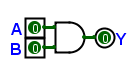
\includegraphics[width=\maxwidth{.95\linewidth}]{gfx/04_01}
	\caption{AND Gate}
	\label{fig:04_01}
\end{figure}

Notice that each input and output is named in order to make it easier to describe the circuit algebraically. In reality, \textsf{AND}  gates are not packaged or sold one at a time; rather, several would be placed on a single \gls{ic}, like the \emph{7408 Quad AND Gate}. The designer would design the circuit card to use whichever of the four gates are needed while leaving the unused gates unconnected. 

There are two common sets of symbols used to represent the various elements in logic diagrams, and whichever is used is of little consequence since the logic is the same. Shaped symbols, as used in Figure \ref{fig:04_01}, are more common in the United States; but the \gls{ieee} has its own symbols which are sometimes used, especially in Europe. Figure \ref{fig:04_02} illustrates the circuit in Figure \ref{fig:04_01} using \gls{ieee} symbols:

% Pull Quote - Marginal Note - Sidebar
\marginpar{In this book, only shaped symbols will be used.}

\begin{figure}[H]
	\centering
	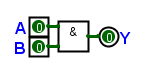
\includegraphics[width=\maxwidth{.95\linewidth}]{gfx/04_02}
	\caption{AND Gate Using IEEE Symbols}
	\label{fig:04_02}
\end{figure}

As an example of an \textsf{AND}  gate at work, consider an elevator: if the door is closed (logic $ 1 $) \textsf{AND} someone in the elevator car presses a floor button (logic $ 1 $), THEN the elevator will move (logic $ 1 $). If both sensors (door and button) are input to an \textsf{AND}  gate, then the elevator motor will only operate if the door is closed \textsf{AND}  someone presses a floor button. 

\subsection{OR}
\label{BF:subsec:or}

An \textsf{OR}  gate is a Boolean operation that will output a logical one, or \emph{True}, if any or all of the inputs are \emph{True}. As an example, consider this statement: ``If my dog needs a bath OR I am going swimming, then I will put on a bathing suit.'' In this statement, ``if my dog needs a bath'' is one input variable and ``I am going swimming'' is another input variable. If either of these is \emph{True}, then the output variable, ``I will put on a bathing suit,'' will also be \emph{True}. However, if both of the inputs are \emph{False}, then the output will also be \emph{False} (or, ``I will not put on a bathing suit''). If you think it odd that I would wear a bathing suit to bathe my dog then you have obviously never met my dog. 

When written in an equation, the Boolean \textsf{OR}  term is represented a number of different ways. One method is to use the logic \textsf{OR}  symbol, as found in Equation \ref{BF:eq:or_vee}.

\begin{align}
  \label{BF:eq:or_vee}
  A \vee B &= Y 
\end{align}

A more common method is to use the \emph{plus} sign that is used for addition in traditional algebra, as in Equation \ref{BF:eq:or_plus}.

\begin{align}
  \label{BF:eq:or_plus}
  A + B &= Y 
\end{align}

For simplicity, the mathematical \emph{plus} symbol is normally used to indicate \textsf{OR}  in printed material since it is easy to enter with a keyboard; however, if there is any chance for ambiguity, then the logic \textsf{OR}  symbol ($ \vee $) is used to differentiate between addition and logic \textsf{OR}.

Table \ref{BF:tab:truth_table_for_or} is the truth table for an \textsf{OR}  operation.

%******************************************************
% OR Truth Table
%******************************************************
\begin{table}[H]
  \sffamily
  \newcommand{\head}[1]{\textcolor{white}{\textbf{#1}}}    
  \begin{center}
    \rowcolors{2}{gray!10}{white} % Color every other line a light gray
    \begin{tabular}{ccc} 
      \rowcolor{black!75}
      \multicolumn{2}{c}{\head{Inputs}} & \head{Output} \\
      A & B & Y \\
      \hline
      0 & 0 & 0 \\
      0 & 1 & 1 \\
      1 & 0 & 1 \\
      1 & 1 & 1 
    \end{tabular}
  \end{center}
  \caption{Truth Table for OR}
  \label{BF:tab:truth_table_for_or}
\end{table}

Notice for the \textsf{OR} truth table that the output is \emph{True} ($ 1 $) whenever at least one input is \emph{True}. Therefore, it could be said that one \emph{True} input would activate an \textsf{OR} Gate. In the following diagram, the input variables $ A $ and $ B $ are wired to an \textsf{OR}  gate, and the output from that gate goes to $ Y $. 

\begin{figure}[H]
	\centering
	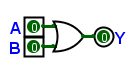
\includegraphics[width=\maxwidth{.95\linewidth}]{gfx/04_03}
	\caption{OR Gate}
	\label{fig:04_03}
\end{figure}

As an example of an \textsf{OR} gate at work, consider a traffic signal. Suppose an intersection is set up such that the light for the main road is normally green; however, if a car pulls up to the intersection from the crossroad, or if a pedestrian presses the ``cross'' button, then the main light is changed to red to stop traffic. This could be done with a simple \textsf{OR} gate. An automobile sensor on the crossroad would be one input and the pedestrian ``cross'' button would be the other input; the output of the \textsf{OR}  gate connecting these two inputs would change the light to red when either input is activated.

\subsection{NOT}
\label{BF:subsec:not}

\textsf{NOT} (or \emph{inverter}) is a Boolean operation that inverts the input. That is, if the input is \emph{True} then the output will be \emph{False} or if the input is \emph{False} then the output will be \emph{True}. When written in an equation, the Boolean \textsf{NOT}  operator is represented in many ways, though two are most popular. The older method is to overline (that is, a line above) a term, or group of terms, that are to be inverted, as in Equation \ref{BF:eq:not_bar}.\marginpar{Equation \ref{BF:eq:not_bar} is read \emph{A OR B NOT = Q} (notice that when spoken, the word \emph{not} follows the term that is inverted).}

\begin{align}
  \label{BF:eq:not_bar}
  A + \overline{B} &= Y 
\end{align}

Another method of indicating \textsf{NOT}  is to use the algebra \emph{prime} indicator, an apostrophe, as in Equation \ref{BF:eq:not_apostrophe}.

\begin{align}
  \label{BF:eq:not_apostrophe}
  A + B' &= Y 
\end{align}

The reason that \textsf{NOT} is most commonly indicated with an apostrophe is because that is easier to enter on a computer keyboard. There are many other ways authors use to represent \textsf{NOT}  in a formula, but none are considered standardized. For example, some authors use an exclamation point: $ A+!B=Q $, others use a broken line: $ A+ \neg B=Q $, others use a backslash: $ A+ \backslash B=Q $, and still others use a tilde: $ A+ \sim B =Q $. However, only the apostrophe and overline are consistently used to indicate \textsf{NOT}. Table \ref{BF:tab:truth_table_for_not} is the truth table for \textsf{NOT}:

%******************************************************
% NOT Truth Table
%******************************************************
\begin{table}[H]
  \sffamily
  \newcommand{\head}[1]{\textcolor{white}{\textbf{#1}}}    
  \begin{center}
    \rowcolors{2}{gray!10}{white} % Color every other line a light gray
    \begin{tabular}{ccc} 
      \rowcolor{black!75}
      \head{Input} & \head{Output} \\
      0 & 1 \\
      1 & 0 \\
    \end{tabular}
  \end{center}
  \caption{Truth Table for NOT}
  \label{BF:tab:truth_table_for_not}
\end{table}

In a logic diagram, \textsf{NOT}  is represented by a small triangle with a ``bubble'' on the output. In Figure \ref{fig:04_04}, the input variable $ A $ is inverted by a \textsf{NOT}  gate and then sent to output $ Y $. 

\begin{figure}[H]
	\centering
	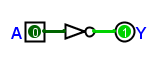
\includegraphics[width=\maxwidth{.95\linewidth}]{gfx/04_04}
	\caption{NOT Gate}
	\label{fig:04_04}
\end{figure}


%*********************************************************************
% NAND Gate
%*********************************************************************
\section{Secondary Logic Functions}
\label{BF:sec:secondary_logic_functions}
\subsection{NAND}
\label{BF:subsec:nand}

\textsf{NAND} is a Boolean operation that outputs the opposite of \textsf{AND}, that is, \textsf{NOT AND}; thus, it will output a logic \emph{False} only if all of the inputs are \emph{True}. The \textsf{NAND} operation is not often used in Boolean equations, but when necessary it is represented by a vertical line. Equation \ref{BF:eq:nand_symbol} shows a \textsf{NAND}  operation.

\begin{align}
  \label{BF:eq:nand_symbol}
  A | B &= Y 
\end{align}

Table \ref{BF:tab:truth_table_for_nand_gate} is the Truth Table for a \textsf{NAND}  gate.

%******************************************************
% NAND Truth Table
%******************************************************
\begin{table}[H]
  \sffamily
  \newcommand{\head}[1]{\textcolor{white}{\textbf{#1}}}    
  \begin{center}
    \rowcolors{2}{gray!10}{white} % Color every other line a light gray
    \begin{tabular}{ccc} 
      \rowcolor{black!75}
      \multicolumn{2}{c}{\head{Inputs}} & \head{Output} \\
      A & B & Y \\
      \hline
      0 & 0 & 1 \\
      0 & 1 & 1 \\
      1 & 0 & 1 \\
      1 & 1 & 0 
    \end{tabular}
  \end{center}
  \caption{Truth Table for \textsf{NAND}  Gate}
  \label{BF:tab:truth_table_for_nand_gate}
\end{table}

In Figure \ref{fig:04_05}, the input variables $ A $ and $ B $ are wired to a NAND gate, and the output from that gate goes to $ Y $.

\begin{figure}[H]
	\centering
	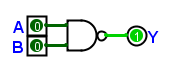
\includegraphics[width=\maxwidth{.95\linewidth}]{gfx/04_05}
	\caption{NAND Gate}
	\label{fig:04_05}
\end{figure}


\marginpar{Inverting bubbles are never found by themselves on a wire; they are always associated with either the inputs or output of a logic gate. To invert a signal on a wire, a \textsf{NOT} gate is used.}The logic diagram symbol for a \textsf{NAND}  gate looks like an \textsf{AND} gate, but with a small bubble on the output port. A bubble in a logic diagram always represents some sort of signal inversion, and it can appear at the inputs or outputs of nearly any logic gate. For example, the bubble on a \textsf{NAND}  gate could be interpreted as ``take whatever the output would be generated by an \textsf{AND} gate\textemdash then invert it.'' 

%*************************************************************
% NOR Gate
%*************************************************************
\subsection{NOR}
\label{BF:subsec:nor}

\textsf{NOR}  is a Boolean operation that is the opposite of OR, that is, \textsf{NOT OR}; thus, it will output a logic \emph{True} only if all of the inputs are \emph{False}. The \textsf{NOR} operation is not often used in Boolean equations, but when necessary it is represented by a downward-pointing arrow. Equation \ref{BF:eq:nor_symbol} shows a \textsf{NOR} operation.

\begin{align}
  \label{BF:eq:nor_symbol}
  A \downarrow B &= Y 
\end{align}

Table \ref{BF:tab:truth_table_for_nor} is the truth table for \textsf{NOR} . 

%******************************************************
% NOR Truth Table
%******************************************************
\begin{table}[H]
  \sffamily
  \newcommand{\head}[1]{\textcolor{white}{\textbf{#1}}}    
  \begin{center}
    \rowcolors{2}{gray!10}{white} % Color every other line a light gray
    \begin{tabular}{ccc} 
      \rowcolor{black!75}
      \multicolumn{2}{c}{\head{Inputs}} & \head{Output} \\
      A & B & Y \\
      \hline
      0 & 0 & 1 \\
      0 & 1 & 0 \\
      1 & 0 & 0 \\
      1 & 1 & 0 
    \end{tabular}
  \end{center}
  \caption{Truth Table for NOR}
  \label{BF:tab:truth_table_for_nor}
\end{table}

In Figure \ref{fig:04_06}, the input variables $ A $ and $ B $ are wired to a \textsf{NOR}  gate, and the output from that gate goes to $ Y $. 

\begin{figure}[H]
	\centering
	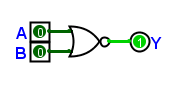
\includegraphics[width=\maxwidth{.95\linewidth}]{gfx/04_06}
	\caption{NOR Gate}
	\label{fig:04_06}
\end{figure}


\subsection{XOR}
\label{BF:subsec:xor}

\textsf{XOR} (\emph{Exclusive OR}) is a Boolean operation that outputs a logical one, or \emph{True}, only if the two inputs are different. This is useful for circuits that compare inputs; if they are different then the output is \emph{True}, otherwise it is \emph{False}. Because of this, an \textsf{XOR}  gate is sometimes referred to as a \emph{Difference Gate}. The \textsf{XOR} operation is not often used in Boolean equations, but when necessary it is represented by a plus sign (like the OR function) inside a circle. Equation \ref{BF:eq:xor_symbol} shows an \textsf{XOR}  operation.

% XOR in equation
\begin{align}
  \label{BF:eq:xor_symbol}
  A \oplus B &= Y
\end{align}

Table \ref{BF:tab:truth_table_for_xor} is the truth table for an \textsf{XOR}  gate.

%******************************************************
% XOR Truth Table
%******************************************************
\begin{table}[H]
  \sffamily
  \newcommand{\head}[1]{\textcolor{white}{\textbf{#1}}}    
  \begin{center}
    \rowcolors{2}{gray!10}{white} % Color every other line a light gray
    \begin{tabular}{ccc} 
      \rowcolor{black!75}
      \multicolumn{2}{c}{\head{Inputs}} & \head{Output} \\
      A & B & Y \\
      \hline
      0 & 0 & 0 \\
      0 & 1 & 1 \\
      1 & 0 & 1 \\
      1 & 1 & 0 
    \end{tabular}
  \end{center}
  \caption{Truth Table for XOR}
  \label{BF:tab:truth_table_for_xor}
\end{table}

In Figure \ref{fig:04_07}, the input variables $ A $ and $ B $ are wired to an \textsf{XOR}  gate, and the output from that gate goes to $ Y $. 

\begin{figure}[H]
	\centering
	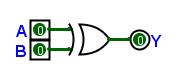
\includegraphics[width=\maxwidth{.95\linewidth}]{gfx/04_07}
	\caption{XOR Gate}
	\label{fig:04_07}
\end{figure}


There is some debate about the proper behavior of an \textsf{XOR}  gate that has more than two inputs. Some experts believe that an \textsf{XOR} gate should output a \emph{True} if one, and only one, input is \emph{True} regardless of the number of inputs. This would seem to be in keeping with the rules of digital logic developed by George Boole and other early logisticians and is the strict definition of \textsf{XOR} promulgated by the \gls{ieee}. This is also the behavior of the \textsf{XOR} gate found in \textit{Logisim-evolution}, the digital logic simulator used in the lab manual accompanying this text. Others believe, though, that an \textsf{XOR} gate should output a \emph{True} if an odd number of inputs is \emph{True}. in \Le this type of behavior is found in a device called a ``parity gate'' and is covered in more detail elsewhere in this book.

%**********************************************************
% XNOR Gate
%**********************************************************
\subsection{XNOR}
\label{BF:subsec:xnor}

\textsf{XNOR} is a Boolean operation that will output a logical one, or \emph{True}, only if the two inputs are the same; thus, an \textsf{XNOR} gate is often referred to as an \emph{Equivalence Gate}. The \textsf{XNOR} operation is not often used in Boolean equations, but when necessary it is represented by a dot inside a circle. Equation \ref{BF:eq:xnor_symbol} shows an \textsf{XNOR}  operation. 

% XNOR in equation
\begin{align}
  \label{BF:eq:xnor_symbol}
  A \odot B &= Y
\end{align}

Table \ref{BF:tab:truth_table_for_xnor} is the truth table for \textsf{XNOR} . 

%******************************************************
% XNOR Truth Table
%******************************************************
\begin{table}[H]
  \sffamily
  \newcommand{\head}[1]{\textcolor{white}{\textbf{#1}}}    
  \begin{center}
    \rowcolors{2}{gray!10}{white} % Color every other line a light gray
    \begin{tabular}{ccc} 
      \rowcolor{black!75}
      \multicolumn{2}{c}{\head{Inputs}} & \head{Output} \\
      A & B & Y \\
      \hline
      0 & 0 & 1 \\
      0 & 1 & 0 \\
      1 & 0 & 0 \\
      1 & 1 & 1 
    \end{tabular}
  \end{center}
  \caption{Truth Table for XNOR}
  \label{BF:tab:truth_table_for_xnor}
\end{table}

In Figure \ref{fig:04_08}, the input variables $ A $ and $ B $ are wired to an \textsf{XNOR}  gate, and the output from that gate goes to $ Y $. 

\begin{figure}[H]
	\centering
	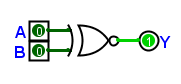
\includegraphics[width=\maxwidth{.95\linewidth}]{gfx/04_08}
	\caption{XNOR Gate}
	\label{fig:04_08}
\end{figure}


\subsection{Buffer}
\label{BF:subsec:buffer}

A buffer (sometimes called \emph{Transfer}) is a Boolean operation that transfers the input to the output without change. If the input is \emph{True}, then the output will be \emph{True} and if the input is \emph{False}, then the output will be \emph{False}. It may seem to be an odd function since this operation does not change anything, but it has an important use in a circuit. As logic circuits become more complex, the signal from input to output may become weak and no longer able to drive (or activate) additional gates. A buffer is used to boost (and stabilize) a logic level so it is more dependable. Another important function for a buffer is to clean up an input signal. As an example, when an electronic circuit interacts with the physical world (such as a user pushing a button), there is often a very brief period when the signal from that physical device waivers between high and low unpredictably. A buffer can smooth out that signal so it is a constant high or low without voltage spikes in between. 

Table \ref{BF:tab:truth_table_for_a_buffer} is the truth table for buffer.

%******************************************************
% Buffer Truth Table
%******************************************************
\begin{table}[H]
  \sffamily
  \newcommand{\head}[1]{\textcolor{white}{\textbf{#1}}}    
  \begin{center}
    \rowcolors{2}{gray!10}{white} % Color every other line a light gray
    \begin{tabular}{ccc} 
      \rowcolor{black!75}
      \head{Input} & \head{Output} \\
      0 & 0 \\
      1 & 1 
    \end{tabular}
  \end{center}
  \caption{Truth Table for a Buffer}
  \label{BF:tab:truth_table_for_a_buffer}
\end{table}

Buffers are rarely used in schematic diagrams since they do not actually change a signal; however, Figure \ref{fig:04_09}, illustrates a buffer. 

\begin{figure}[H]
	\centering
	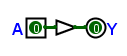
\includegraphics[width=\maxwidth{.95\linewidth}]{gfx/04_09}
	\caption{Buffer}
	\label{fig:04_09}
\end{figure}

\section{Univariate Boolean Algebra Properties}
\label{BF:sec:univariate_boolean_algebra_properties}
\subsection{Introduction}
\label{BF:subsec:introduction_to_univariate}

Boolean Algebra, like real number algebra, includes a number of properties. This unit introduces the univariate Boolean properties, or those properties that involve only one input variable. These properties permit Boolean expressions to be simplified, and circuit designers are interested in simplifying circuits to reduce construction expense, power consumption, heat loss (wasted energy), and troubleshooting time.  

\subsection{Identity}
\label{BF:subsec:identity}

In mathematics, an identity is an equality where the left and right members are the same regardless of the values of the variables present. As an example, Equation \ref{BF:eq:identity_example} is an identity since the two members are identical regardless of the value of $ \alpha $:

\begin{align}
  \label{BF:eq:identity_example}
  \frac{\alpha}{2} &= 0.5\alpha
\end{align}

An \emph{Identity Element} is a special member of a set such that when that element is used in a binary operation the other element in that operation is not changed. This is sometimes called the \emph{Neutral Element} since it has no effect on binary operations. As an example, in Equation \ref{BF:eq:identity_element_of_addition} the two members of the equation are always identical. Therefore, zero is the identity element for addition since anything added to zero remains unchanged.

\begin{align}
  \label{BF:eq:identity_element_of_addition}
  a + 0 &= a 
\end{align}

In a logic circuit, combining any logic input with a logic zero through an \textsf{OR}  gate yields the original input. Logic zero, then, is considered the \textsf{OR} identity element because it causes the input of the gate to be copied to the output unchanged. Because \textsf{OR}  is represented by a plus sign when written in a Boolean equation, and the identity element for \textsf{OR}  is zero, Equation \ref{BF:eq:or_identity} is \emph{True}.

\begin{align}
  \label{BF:eq:or_identity}
  A + 0 &= A 
\end{align}

The bottom input to the \textsf{OR} gate in \ref{fig:04_10} is a constant logic zero, or \emph{False}. The output for this circuit, $ Y $, will be the same as input $ A $; therefore, the identity element for \textsf{OR}  is zero.  

\begin{figure}[H]
	\centering
	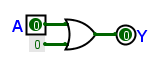
\includegraphics[width=\maxwidth{.95\linewidth}]{gfx/04_10}
	\caption{OR Identity Element}
	\label{fig:04_10}
\end{figure}

In the same way, combining any logic input with a logic one through an \textsf{AND}  gate yields the original input. Logic one, then, is considered the \textsf{AND}  identity element because it causes the input of the gate to be copied to the output unchanged. Because \textsf{AND}  is represented by a multiplication sign when written in a Boolean equation, and the identity element for \textsf{AND} is one, Equation \ref{BF:eq:and_identity} is \emph{True}.

\begin{align}
  \label{BF:eq:and_identity}
  A * 1 &= A 
\end{align}

The bottom input to the \textsf{AND} gate in \ref{fig:04_11} is a constant logic one, or \emph{True}. The output for this circuit, $ Y $, will be the same as input $ A $; therefore, the identity element for \textsf{AND}  is one.  

\begin{figure}[H]
	\centering
	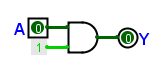
\includegraphics[width=\maxwidth{.95\linewidth}]{gfx/04_11}
	\caption{AND Identity Element}
	\label{fig:04_11}
\end{figure}

\subsection{Idempotence}
\label{BF:subsec:idempotence}

If the two inputs of either an \textsf{OR} or \textsf{AND} gate are tied together, then the same signal will be applied to both inputs. This results in the output of either of those gates being the same as the input; and this is called the idempotence property. An electronic gate wired in this manner performs the same function as a buffer. 

% Pull Quote - Marginal Note - Sidebar
\marginpar{Remember that in Boolean expressions a plus sign represents an \textsf{OR}  gate, not mathematical addition.}

\begin{align}
  \label{BF:eq:idempotence_for_or}
  A + A &= A 
\end{align}

\begin{figure}[H]
	\centering
	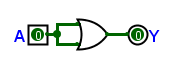
\includegraphics[width=\maxwidth{.95\linewidth}]{gfx/04_12}
	\caption{Idempotence Property for OR Gate}
	\label{fig:04_12}
\end{figure}

Figure \ref{fig:04_12} illustrates the idempotence property for an \textsf{AND} gate.

% Pull Quote - Marginal Note - Sidebar
\marginpar{Remember that in a Boolean expression a multiplication sign represents an AND gate, not mathematical multiplying.}

\begin{align}
  \label{BF:eq:idempotence_for_and}
  A * A &= A 
\end{align}

\begin{figure}[H]
	\centering
	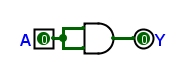
\includegraphics[width=\maxwidth{.95\linewidth}]{gfx/04_13}
	\caption{Idempotence Property for AND Gate}
	\label{fig:04_13}
\end{figure}

\subsection{Annihilator}
\label{BF:subsec:annihilator}

Combining any data and a logic one through an \textsf{OR} gate yields a constant output of one. This property is called the annihilator since the \textsf{OR} gate outputs a constant one; in other words, whatever other data were input are lost. Because \textsf{OR} is represented by a plus sign when written in a Boolean equation, and the annihilator for \textsf{OR} is one, the following is true:

\begin{align}
  \label{BF:eq:annihilator_or}
  A + 1 &= 1 
\end{align}

\begin{figure}[H]
	\centering
	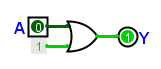
\includegraphics[width=\maxwidth{.95\linewidth}]{gfx/04_14}
	\caption{Annihilator For OR Gate}
	\label{fig:04_14}
\end{figure}

The bottom input for the \textsf{OR}  gate in Figure \ref{fig:04_14} is a constant logic one, or \emph{True}. The output for this circuit will be \emph{True} (or $ 1 $) no matter whether input $ A $ is \emph{True} or \emph{False} ($ 1 $ or $ 0 $).

Combining any data and a logic zero with an \textsf{AND} gate yields a constant output of zero. This property is called the annihilator since the \textsf{AND}  gate outputs a constant zero; in other words, whatever logic data were input are lost. Because \textsf{AND}  is represented by a multiplication sign when written in a Boolean equation, and the annihilator for \textsf{AND} is zero, the following is true:

\begin{align}
  \label{BF:eq:annihilator_and}
  A * 0 &= 0 
\end{align}

\begin{figure}[H]
	\centering
	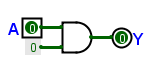
\includegraphics[width=\maxwidth{.95\linewidth}]{gfx/04_15}
	\caption{Annihilator For AND Gate}
	\label{fig:04_15}
\end{figure}

The bottom input for the \textsf{AND} gate in Figure \ref{fig:04_15} is a constant logic zero, or \emph{False}. The output for this circuit will be \emph{False} (or $ 0 $) no matter whether input $ A $ is \emph{True} or \emph{False} ($ 1 $ or $ 0 $).

\subsection{Complement}
\label{BF:subsec:complement}

In Boolean logic there are only two possible values for variables: $ 0 $ and $ 1 $. Since either a variable or its complement must be one, and since combining any data with one through an \textsf{OR} gate yields one (see the Annihilator in Equation \ref{BF:eq:annihilator_or}), then the following is true:

\begin{align}
  \label{BF:eq:complement_or}
  A + A' &= 1 
\end{align}

\begin{figure}[H]
	\centering
	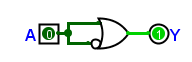
\includegraphics[width=\maxwidth{.95\linewidth}]{gfx/04_16}
	\caption{OR Complement}
	\label{fig:04_16}
\end{figure}

In Figure \ref{fig:04_16}, the output ($ Y $) will always equal one, regardless of the value of input $ A $. This leads to the general property that when a variable and its complement are combined through an \textsf{OR} gate the output will always be one. 

In the same way, since either a variable or its complement must be zero, and since combining any data with zero through an \textsf{AND} gate yields zero (see the Annihilator in Equation \ref{BF:eq:annihilator_and}), then the following is true: 

\begin{align}
  \label{BF:eq:complement_and}
  A * A' &= 0
\end{align}

\begin{figure}[H]
	\centering
	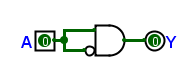
\includegraphics[width=\maxwidth{.95\linewidth}]{gfx/04_17}
	\caption{AND Complement}
	\label{fig:04_17}
\end{figure}

\subsection{Involution}
\label{BF:subsec:involution}

\marginpar{The Involution Property is sometimes called the ``Double Complement'' Property.}

Another law having to do with complementation is that of Involution. Complementing a Boolean variable two times (or any even number of times) results in the original Boolean value. 

\begin{align}
  \label{BF:eq:involuton}
  (A')' &= A
\end{align}

\begin{figure}[H]
	\centering
	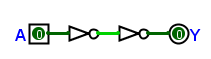
\includegraphics[width=\maxwidth{.95\linewidth}]{gfx/04_18}
	\caption{Involution Property}
	\label{fig:04_18}
\end{figure}

In the circuit illustrated in Figure \ref{fig:04_18}, the output ($ Y $) will always be the same as the input ($ A $). 

% Begin Sidebar Box
\begin{tcolorbox}[colback=blue!5!white,colframe=blue!75!black]
  % Upper half of box: my "title" area
  \textcolor{blue}{\textbf{Propagation Delay}}
  % Lower half of the box: the content
  \tcblower
  It takes the two \textsf{NOT} gates a short period of time to pass a signal from input to output, which is known as ``propagation delay.'' A designer occasionally needs to build an intentional signal delay into a circuit for some reason and two (or any even number of) consecutive \textsf{NOT} gates would be one option.
\end{tcolorbox}
% End Sidebar Box

\section{Multivariate Boolean Algebra Properties}
\label{BF:sec:multivariate_boolean_algebra_properties}
\subsection{Introduction}
\label{BF:subsec:introduction_to_multivariate}

Boolean Algebra, like real number algebra, includes a number of properties. This unit introduces the multivariate Boolean properties, or those properties that involve more than one input variable. These properties permit Boolean expressions to be simplified, and circuit designers are interested in simplifying circuits to reduce construction expense, power consumption, heat loss (wasted energy), and troubleshooting time.  

\subsection{Commutative}
\label{BF:subsec:commutative_property}

\marginpar{The examples here show only two variables, but this property is true for any number of variables.}

In essence, the commutative property indicates that the order of the input variables can be reversed in either \textsf{OR} or \textsf{AND} gates without changing the truth of the expression. Equation \ref{BF:eq:commutative} expresses this property algebraically.

\begin{align}
  \label{BF:eq:commutative}
  A + B &= B + A \\
  \nonumber
  A * B &= B * A
\end{align}

\begin{figure}[H]
	\centering
	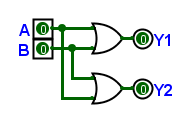
\includegraphics[width=\maxwidth{.95\linewidth}]{gfx/04_19}
	\caption{Commutative Property for OR}
	\label{fig:04_19}
\end{figure}

\marginpar{\textsf{XOR} and \textsf{XNOR} are also commutative; but for only two variables, not three or more.}

\begin{figure}[H]
	\centering
	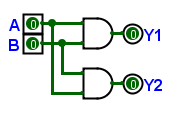
\includegraphics[width=\maxwidth{.95\linewidth}]{gfx/04_20}
	\caption{Commutative Property for AND}
	\label{fig:04_20}
\end{figure}

In Figures \ref{fig:04_19} and \ref{fig:04_20} the inputs are reversed for the two gates, but the outputs are the same. For example, $ A $ is entering the top input for the upper \textsf{OR} gate, but the bottom input for the lower gate; however, $ Y1 $ is always equal to $ Y2 $.

\subsection{Associative}
\label{BF:subsec:associative_property}

\marginpar{The examples here show only three variables, but this property is true for any number of variables.}

This property indicates that groups of variables in an \textsf{OR} or \textsf{AND} gate can be associated in various ways without altering the truth of the equations. Equation \ref{BF:eq:associative} expresses this property algebraically: 

\begin{align}
  \label{BF:eq:associative}
  ( A + B ) + C &= A + ( B + C ) \\
  \nonumber
  ( A * B ) * C &= A * ( B * C )
\end{align}

\marginpar{\textsf{XOR} and \textsf{XNOR} are also associative; but for only two variables, not three or more.}

In the circuits in Figure \ref{fig:04_21} and \ref{fig:04_22} , notice that $ A $ and $ B $ are associated together in the first gate, and then $ C $ is associated with the output of that gate. Then, in the lower half of the circuit, $ B $ and $ C $ are associated together in the first gate, and then $ A $ is associated with the output of that gate. Since $ Y1 $ is always equal to $ Y2 $ for any combination of inputs, it does not matter which of the two variables are associated together in a group of gates.  

\begin{figure}[H]
	\centering
	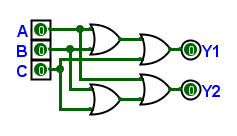
\includegraphics[width=\maxwidth{.95\linewidth}]{gfx/04_21}
	\caption{Associative Property for OR}
	\label{fig:04_21}
\end{figure}

\begin{figure}[H]
	\centering
	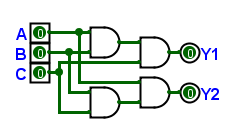
\includegraphics[width=\maxwidth{.95\linewidth}]{gfx/04_22}
	\caption{Associative Property for AND}
	\label{fig:04_22}
\end{figure}

\subsection{Distributive}
\label{BF:subsec:distributive_property}

The distributive property of real number algebra permits certain variables to be ``distributed'' to other variables. This operation is frequently used to create groups of variables that can be simplified; thus, simplifying the entire expression. Boolean algebra also includes a distributive property, and that can be used to combine \textsf{OR}  or \textsf{AND}  gates in various ways that make it easier to simplify the circuit. Equation \ref{BF:eq:distributive} expresses this property algebraically:

\begin{align}
  \label{BF:eq:distributive}
  A( B + C ) &= AB + AC \\
  \nonumber
  A + (BC) &= (A + B) (A + C)
\end{align}

In the circuits illustrated in Figures \ref{fig:04_23} and \ref{fig:04_24}, notice that input $ A $ in the top half of the circuit is distributed to inputs $ B $ and $ C $ in the bottom half. However, output $ Y1 $ is always equal to output $ Y2 $ regardless of how the inputs are set. These two circuits illustrate Distributive of \textsf{AND} over \textsf{OR}  and Distributive of \textsf{OR} over \textsf{AND} .
 
\begin{figure}[H]
	\centering
	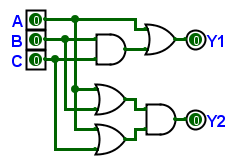
\includegraphics[width=\maxwidth{.95\linewidth}]{gfx/04_23}
	\caption{Distributive Property for AND over OR}
	\label{fig:04_23}
\end{figure}

\begin{figure}[H]
	\centering
	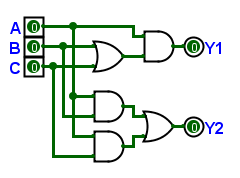
\includegraphics[width=\maxwidth{.95\linewidth}]{gfx/04_24}
	\caption{Distributive Property for OR over AND}
	\label{fig:04_24}
\end{figure}

\subsection{Absorption}
\label{BF:subsec:absorption_property}

The absorption property is used to remove logic gates from a circuit if those gates have no effect on the output. In essence, a gate is ``absorbed'' if it is not needed. There are two different absorption properties:

\begin{align}
  \label{BF:eq:absorption}
  A + (AB) &= A \\
  \nonumber
  A(A + B) &= A
\end{align}

The best way to think about why these properties are true is to imagine a circuit that contains them. The first circuit below illustrates the top equation. 

\begin{figure}[H]
	\centering
	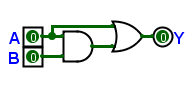
\includegraphics[width=\maxwidth{.95\linewidth}]{gfx/04_25}
	\caption{Absorption Property (Version 1)}
	\label{fig:04_25}
\end{figure}

Table \ref{BF:tab:truth_table_for_absorption_property_version_1} is the truth table for the circuit in Figure \ref{fig:04_25}.

%******************************************************
% Absorption (Version 1) Truth Table
%******************************************************
\begin{table}[H]
  \sffamily
  \newcommand{\head}[1]{\textcolor{white}{\textbf{#1}}}    
  \begin{center}
    \rowcolors{2}{gray!10}{white} % Color every other line a light gray
    \begin{tabular}{ccc} 
      \rowcolor{black!75}
      \multicolumn{2}{c}{\head{Inputs}} & \head{Output} \\
      A & B & Y \\
      \hline
      0 & 0 & 0 \\
      0 & 1 & 0 \\
      1 & 0 & 1 \\
      1 & 1 & 1 
    \end{tabular}
  \end{center}
  \caption{Truth Table for Absorption Property}
  \label{BF:tab:truth_table_for_absorption_property_version_1}
\end{table}

Notice that the output, $ Y $, is always the same as input $ A $. This means that input $ B $ has no bearing on the output of the circuit; therefore, the circuit could be replaced by a piece of wire from input $ A $ to output $ Y $. Another way to state that is to say that input $ B $ is absorbed by the circuit.

The circuit illustrated in Figure \ref{fig:04_26} is the second version of the Absorption Property. Like the first Absorption Property circuit, a truth table would demonstrate that input $ B $ is absorbed by the circuit. 

\begin{figure}[H]
	\centering
	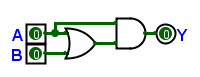
\includegraphics[width=\maxwidth{.95\linewidth}]{gfx/04_26}
	\caption{Absorption Property (Version 2)}
	\label{fig:04_26}
\end{figure}

\subsection{Adjacency}
\label{BF:subsec:adjacency_property}

The adjacency property simplifies a circuit by removing unnecessary gates.

\begin{align}
  \label{BF:eq:adjacency}
  AB + AB' &= A
\end{align}

This property can be proven by simple algebraic manipulation:

\begin{align}
  \label{BF:eq:adjacency_solved}
  AB + AB' && \text{Original Expression} \\
  \nonumber
  A ( B + B') && \text{Distributive Property} \\
  \nonumber
  A1 && \text{Complement Property} \\
  \nonumber
  A && \text{Identity Element}
\end{align}

The circuit in Figure \ref{fig:04_27} illustrates the adjacency property. If this circuit were constructed it would be seen that the output, $ Y $, is always the same as input $ A $; therefore, this entire circuit could be replaced by a single wire from input $ A $ to output $ Y $.

\begin{figure}[H]
	\centering
	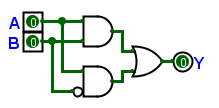
\includegraphics[width=\maxwidth{.95\linewidth}]{gfx/04_27}
	\caption{Adjacency Property}
	\label{fig:04_27}
\end{figure}

\section{DeMorgan's Theorem}
\label{BF:sec:demorgans_theorem}
\subsection{Introduction}
\label{BF:subsec:introduction_demorgans}

A mathematician named Augustus DeMorgan developed a pair of important theorems regarding the complementation of groups in Boolean algebra. DeMorgan found that an \textsf{OR} gate with all inputs inverted (a Negative-\textsf{OR} gate) behaves the same as a \textsf{NAND}  gate with non-inverted inputs; and an \textsf{AND} gate with all inputs inverted (a Negative-\textsf{AND} gate) behaves the same as a \textsf{NOR} gate with non-inverted inputs. DeMorgan's theorem states that inverting the output of any gate is the same as using the opposite type of gate with inverted inputs. Figure \ref{fig:04_28} illustrates this in circuit terms: the \textsf{NAND} gate with normal inputs and the \textsf{OR} gate with inverted inputs are functionally equivalent; that is, $ Y1 $ will always equal $ Y2 $, regardless of the values of input $ A $ or $ B $.  

\begin{figure}[H]
	\centering
	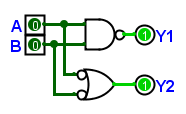
\includegraphics[width=\maxwidth{.95\linewidth}]{gfx/04_28}
	\caption{DeMorgan's Theorem Defined}
	\label{fig:04_28}
\end{figure}

The NOT function is commonly represented in an equation as an apostrophe because it is easy to enter with a keyboard, like: $ (AB)' $ for \emph{A AND B NOT}. However, it is easiest to work with DeMorgan's theorem if \textsf{NOT} is represented by an overline rather than an apostrophe, so it would be written as $ \overline{AB} $ rather than $ (AB)' $. Remember that an overline is a grouping symbol (like parenthesis) and it means that everything under that bar would first be combined (using an \textsf{AND} or \textsf{OR} gate) and then the output of the combination would be complemented.

\subsection{Applying DeMorgan's Theorem}
\label{BF:subsec:applying_demorgans_theorem}

Applying DeMorgan's theorem to a Boolean expression may be thought of in terms of \emph{breaking the bar}. When applying DeMorgan's theorem to a Boolean expression:

\begin{enumerate}
\item A complement bar is broken over a group of variables.
\item The operation (\textsf{AND}  or \textsf{OR} ) directly underneath the broken bar changes.
\item Pieces of the broken bar remain over the individual variables. 
\end{enumerate}

To illustrate:

\begin{align}
  \label{BF:eq:demorgan_nand}
  \overline{A*B} \leftrightarrow \overline{A}+\overline{B}
\end{align}

\begin{align}
  \label{BF:eq:demorgan_nor}
  \overline{A+B} \leftrightarrow \overline{A}*\overline{B}
\end{align}

Equation \ref{BF:eq:demorgan_nand} shows how a two-input \textsf{NAND} gate is ``broken'' to form an \textsf{OR} gate with two inverted inputs and equation \ref{BF:eq:demorgan_nor} shows how a two-input \textsf{NOR} gate is ``broken'' to form an \textsf{AND} gate with two complemented inputs.

\subsection{Simple Example}
\label{BF:subsec:simple_example_demorgan}

When multiple ``layers'' of bars exist in an expression, only one bar is broken at a time, and the longest, or uppermost, bar is broken first. As an example, consider the circuit in Figure \ref{fig:04_29}: 

\begin{figure}[H]
	\centering
	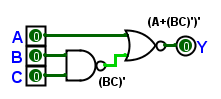
\includegraphics[width=\maxwidth{.95\linewidth}]{gfx/04_29}
	\caption{DeMorgan's Theorem Example 1}
	\label{fig:04_29}
\end{figure}

By writing the output at each gate (as illustrated in Figure \ref{fig:04_29}), it is easy to determine the Boolean expression for the circuit. Note: all circuit diagrams in this book are generated with \Le and the text tool in that software does not permit drawing overbars. Therefore, the circuit diagram will use the apostrophe method of indicating NOT but overbars will be used in the text.

\begin{align}
  \label{BF:eq:demorgan_simple_example}
  \overline{A+\overline{BC}}
\end{align}

To simplify the circuit, break the bar covering the entire expression (the ``longest bar''), and then simplify the resulting expression.

\begin{align}
  \label{BF:eq:demorgan_simple_solved}
  \overline{A+\overline{BC}} && \text{Original Expression} \\
  \nonumber
  \overline{A}\,\overline{\overline{BC}} && \text{''Break'' the longer bar} \\
  \nonumber
  \overline{A}BC && \text{Involution Property}
\end{align}

As a result, the original circuit is reduced to a three-input \textsf{AND} gate with one inverted input.

\subsection{Incorrect Application of DeMorgan's Theorem}
\label{BF:subsec:incorrect_application_of_demorgans_theorem}

More than one bar is never broken in a single step, as illustrated in Equation \ref{BF:eq:demorgan_incorrect_solution}: 

\begin{align}
  \label{BF:eq:demorgan_incorrect_solution}
  \overline{A+\overline{BC}} && \text{Original Expression} \\
  \nonumber
  \overline{A\overline{B}}+\overline{\overline{C}} && \text{Improperly Breaking Two Bars} \\
  \nonumber
  \overline{A}B+C && \text{Incorrect Solution}
\end{align}

Thus, as tempting as it may be to take a shortcut and break more than one bar at a time, it often leads to an incorrect result. Also, while it is possible to properly reduce an expression by breaking the short bar first; more steps are usually required and that process is not recommended.  

\subsection{About Grouping}
\label{BF:subsec:demorgans_about_grouping}

An important, but easily neglected, aspect of DeMorgan's theorem concerns grouping. Since a bar functions as a grouping symbol, the variables formerly grouped by a broken bar must remain grouped or else proper precedence (order of operation) will be lost. Therefore, after simplifying a large grouping of variables, it is a good practice to place them in parentheses in order to keep the order of operation the same.  

Consider the circuit in Figure \ref{fig:04_30}.

\begin{figure}[H]
	\centering
	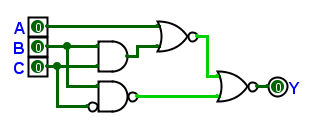
\includegraphics[width=\maxwidth{.95\linewidth}]{gfx/04_30}
	\caption{DeMorgan's Theorem Example 2}
	\label{fig:04_30}
\end{figure}

As always, the first step in simplifying this circuit is to generate the Boolean expression for the circuit, which is done by writing the sub-expression at the output of each gate. That results in Expression \ref{BF:eq:demorgan_grouping_solution}, which is then simplified. 

\begin{align}
  \label{BF:eq:demorgan_grouping_solution}
  \overline{ \overline{A+BC} + \overline{A \overline{B}}} && \text{Original Expression} \\
  \nonumber
  ( \overline{\overline{A+BC}} ) ( \overline{\overline{A\overline{B}}} ) && \text{Breaking the Longest Bar} \\
  \nonumber
  (A+BC)(A\overline{B}) && \text{Involution} \\
  \nonumber
  (AA\overline{B}) (BCA\overline{B}) && \text{Distribute $ A\overline{B} $ to $ (A+BC) $} \\
  \nonumber
  (A\overline{B})+(BCA\overline{B}) && \text{Idempotence: $ AA=A $} \\
  \nonumber
  (A\overline{B})+(0CA)) && \text{Complement: $ B\overline{B}=0 $} \\
  \nonumber
  (A\overline{B})+0 && \text{Annihilator: $ 0CA=0 $} \\
  \nonumber
  A\overline{B} && \text{Identity: $ A+0=A $}
\end{align}

The equivalent gate circuit for this much-simplified expression is as follows:

\begin{figure}[H]
	\centering
	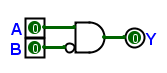
\includegraphics[width=\maxwidth{.95\linewidth}]{gfx/04_31}
	\caption{DeMorgan's Theorem Example 2 Simplified}
	\label{fig:04_31}
\end{figure}

\subsection{Summary}
\label{BF:subsec:demorgans_summary}

Here are the important points to remember about DeMorgan's Theorem: 

\begin{itemize}
  \item It describes the equivalence between gates with inverted inputs and gates with inverted outputs. 
  \item When "breaking" a complementation (or \textsf{NOT}) bar in a Boolean expression, the operation directly underneath the break (\textsf{AND} or \textsf{OR}) reverses and the broken bar pieces remain over the respective terms. 
  \item It is normally easiest to approach a problem by breaking the longest (uppermost) bar before breaking any bars under it. 
  \item Two complementation bars are never broken in one step. 
  \item Complementation bars function as grouping symbols. Therefore, when a bar is broken, the terms underneath it must remain grouped. Parentheses may be placed around these grouped terms as a help to avoid changing precedence.
\end{itemize}

\subsection{Example Problems}
\label{BF:subsec:demorgans_example_problems}

The following examples use DeMorgan's Theorem to simplify a Boolean expression.

%******************************************************
% DeMorgan's Problems
%******************************************************
\begin{table}[H]
  \newcommand{\head}[1]{\textcolor{white}{\textbf{#1}}}    
  \begin{center}
    \rowcolors{2}{gray!10}{white} % Color every other line a light gray
    \begin{tabular}{c|cc} 
      \rowcolor{black!75}
      & \head{Original Expression} & \head{Simplified} \\
      1 & $ (\overline{A+B})(\overline{ABC})(\overline{\overline{A}C}) $ 
        & $ \overline{A}\,\overline{B}\,\overline{C} $ \\
      2 & $ \overline{(AB+\overline{B}C)+(B\overline{C}+\overline{A}B)} $ 
        & $ \overline{B}\,\overline{C} $ \\
      3 & $ (AB+\overline{B}C)(AC+\overline{A}\,\overline{C}) $ 
        & $ \overline{A}+\overline{C} $ 
    \end{tabular}
  \end{center}
  \label{BF:tab:demorgans_example_problems}
  \sffamily
\end{table}

\section{Boolean Functions}
\label{BF:sec:boolean_functions}

Consider Figure \ref{fig:04_32}, which is a generic circuit with two inputs and one output.

\begin{figure}[H]
	\centering
	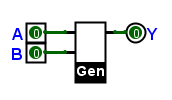
\includegraphics[width=\maxwidth{.95\linewidth}]{gfx/04_32}
	\caption{Generic Function}
	\label{fig:04_32}
\end{figure}

Without knowing anything about what is in the unlabeled box at the center of the circuit, there are a number of possible truth tables which could describe the circuit's output. Two possibilities are shown in Truth Table \ref{BF:tab:truth_table_for_generic_circuit_one} and Truth Table \ref{BF:tab:truth_table_for_generic_circuit_two}.

%******************************************************
% Generic Truth Table 1
%******************************************************
\begin{table}[H]
  \sffamily
  \newcommand{\head}[1]{\textcolor{white}{\textbf{#1}}}    
  \begin{center}
    \rowcolors{2}{gray!10}{white} % Color every other line a light gray
    \begin{tabular}{ccc} 
      \rowcolor{black!75}
      \multicolumn{2}{c}{\head{Inputs}} & \head{Output} \\
      A & B & Y \\
      \hline
      0 & 0 & 0 \\
      0 & 1 & 1 \\
      1 & 0 & 0 \\
      1 & 1 & 1 
    \end{tabular}
  \end{center}
  \caption{Truth Table for Generic Circuit One}
  \label{BF:tab:truth_table_for_generic_circuit_one}
\end{table}

%******************************************************
% Generic Truth Table 2
%******************************************************
\begin{table}[H]
  \sffamily
  \newcommand{\head}[1]{\textcolor{white}{\textbf{#1}}}    
  \begin{center}
    \rowcolors{2}{gray!10}{white} % Color every other line a light gray
    \begin{tabular}{ccc} 
      \rowcolor{black!75}
      \multicolumn{2}{c}{\head{Inputs}} & \head{Output} \\
      A & B & Y \\
      \hline
      0 & 0 & 0 \\
      0 & 1 & 1 \\
      1 & 0 & 1 \\
      1 & 1 & 0 
    \end{tabular}
  \end{center}
  \caption{Truth Table for Generic Circuit Two}
  \label{BF:tab:truth_table_for_generic_circuit_two}
\end{table}

In fact, there are $ 16 $ possible truth tables for this circuit. Each of those truth tables reflect a single potential function of the circuit by setting various combinations of input/output. Therefore, any two-input, one-output circuit has $ 16 $ possible functions. It is easiest to visualize all $ 16 $ combinations of inputs/outputs by using an odd-looking truth table. Consider only one of those $ 16 $ functions, the one for the generic circuit described by Truth Table \ref{BF:tab:truth_table_for_generic_circuit_two}. That function is also found in the Boolean Functions Table \ref{BF:tab:boolean_functions} and one row from that table is reproduced in Table \ref{BF:tab:boolean_function_six}.

\begin{table}[H]
  \sffamily
  \newcommand{\head}[1]{\textcolor{white}{\textbf{#1}}}    
  \begin{center}
    %\rowcolors{2}{gray!10}{white} % Color every other line a light gray
    \begin{tabular}{llllll}
      \textbf{A} & 0 & \cellcolor{gray!10}0 & 1 & 1 &  \\ 
      \textbf{B} & 0 & \cellcolor{gray!10}1 & 0 & 1 &  \\ \hline
      $ F_{6} $ & 0 & \cellcolor{gray!10}1 & 1 & 0 
      & Exclusive Or (XOR): $ A \oplus B $ \\ 
    \end{tabular} 
  \end{center}
  \caption{Boolean Function Six}
  \label{BF:tab:boolean_function_six}
\end{table}

The line shown in Table \ref{BF:tab:boolean_function_six} is for \emph{Function 6}, or $ F_6 $ (note that the pattern of the outputs is $ 0110 $, which is binary $ 6 $). Inputs $ A $ and $ B $ are listed at the top of the table. For example, the highlighted column of the table shows that when $ A $ is zero and $ B $ is one the output is one. Therefore, on the line that defines $ F_6 $, the output is \emph{True} when $ [ (A=0 $ \textsf{AND} $ B=1) $ \textsf{OR} $ (A=1 $ \textsf{AND} $ B=0) ] $ This is an \textsf{XOR} function, and the last column of the table verbally describes that function.   

Table \ref{BF:tab:boolean_functions} is the complete Boolean Function table.

\begin{table}[H]
  \sffamily
  \newcommand{\head}[1]{\textcolor{white}{\textbf{#1}}}    
  \begin{center}
    \rowcolors{2}{gray!10}{white} % Color every other line a light gray
    \begin{tabular}{llllll}
    \textbf{A} & 0 & 0 & 1 & 1 &  \\ 
    \textbf{B} & 0 & 1 & 0 & 1 &  \\ \hline
    $ F_{0} $ & 0 & 0 & 0 & 0 
      & Zero or Clear. Always zero (Annihilation) \\ 
    $ F_{1} $ & 0 & 0 & 0 & 1 
      & Logical AND: $ A * B $  \\ 
    $ F_{2} $ & 0 & 0 & 1 & 0 
      & Inhibition: $ AB' $ or $ A>B $ \\ 
    $ F_{3} $ & 0 & 0 & 1 & 1 
      & Transfer A to Output, Ignore B \\ 
    $ F_{4} $ & 0 & 1 & 0 & 0 
      & Inhibition: $ A'B $ or $ B>A $ \\ 
    $ F_{5} $ & 0 & 1 & 0 & 1 
      & Transfer B to Output, Ignore A \\ 
    $ F_{6} $ & 0 & 1 & 1 & 0 
      & Difference, XOR: $ A \oplus B $ \\ 
    $ F_{7} $ & 0 & 1 & 1 & 1 
      & Logical OR: $ A + B $ \\ 
    $ F_{8} $ & 1 & 0 & 0 & 0 
      & Logical NOR: $ (A + B)' $ \\ 
    $ F_{9} $ & 1 & 0 & 0 & 1 
      & Equivalence, XNOR: $ (A = B)' $ \\ 
    $ F_{10} $ & 1 & 0 & 1 & 0 
      & Not B and ignore A, B Complement \\ 
    $ F_{11} $ & 1 & 0 & 1 & 1 
      & Implication, $ A + B' $, $ B >= A $ \\ 
    $ F_{12} $ & 1 & 1 & 0 & 0 
      & Not A and ignore B, A Complement \\ 
    $ F_{13} $ & 1 & 1 & 0 & 1 
      & Implication, $ A' + B $, $ A >= B $ \\ 
    $ F_{14} $ & 1 & 1 & 1 & 0 
      & Logical NAND: $ (A*B)' $ \\ 
    $ F_{15} $ & 1 & 1 & 1 & 1 
      & One or Set. Always one (Identity) \\ 
    \end{tabular} 
  \end{center}
  \caption{Boolean Functions}
  \label{BF:tab:boolean_functions}
\end{table}

\section{Functional Completeness}
\label{BF:sec:functional_completeness}

A set of Boolean operations is said to be \emph{functionally complete} if every possible Boolean function can be derived from that set. The Primary Logic Operations (page \pageref{BF:sec:primary_logic_operations}) are functionally complete since the Secondary Logic Functions (page \pageref{BF:sec:secondary_logic_functions}) can be derived from them. As an example, Equation \ref{BF:eq:xor_from_and} and Figure \ref{fig:04_33} shows how an \textsf{XOR} function can be derived from only \textsf{AND}, \textsf{OR}, and \textsf{NOT} gates.

% XOR in equation
\begin{align}
  \label{BF:eq:xor_from_and}
  ( (A * B)' * ( A + B) )  &= A \oplus B
\end{align}

\begin{figure}[H]
	\centering
	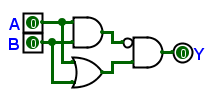
\includegraphics[width=\maxwidth{.95\linewidth}]{gfx/04_33}
	\caption{XOR Derived From AND/OR/NOT}
	\label{fig:04_33}
\end{figure}

While the Primary Operations are functionally complete, it is possible to define other functionally complete sets of operations. For example, using DeMorgan's Theorem, the set of \{\textsf{AND}, \textsf{NOT}\} is also functionally complete since the \textsf{OR}  operation can be defined as $ (A'B')' $. In fact, both \{\textsf{NAND}\} and \{NOR\} operations are functionally complete by themselves. As an example, the \textsf{NOT}  operation can be derived using only \textsf{NAND} gates: $ ( A | A ) $. Because all Boolean functions can be derived from either \textsf{NAND} or \textsf{NOR} operations, these are sometimes considered \emph{universal} operations and it is a common challenge for students to create some complex Boolean function using only one of these two types of operations.